\section{Theoretical Analysis}
\label{sec:analysis}

\subsection{Node analysis method}
\label{sec:node}

\begin{table}[H]
  \centering
  \begin{tabular}{|c|c|}
    \hline
        {\bf Name} & {\bf Value} \\
        \hline
        \hline
        $V_2\;(V)$ & $5.070727$ \\ 
\hline
$V_3\;(V)$ & $4.825468$ \\ 
\hline
$V_4\;(V)$ & $4.304579$ \\ 
\hline
$V_5\;(V)$ & $4.860091$ \\ 
\hline
$V_6\;(V)$ & $8.720760$ \\ 
\hline
$V_7\;(V)$ & $-2.939898$ \\ 
\hline
$V_8\;(V)$ & $-1.950198$ \\ 
\hline
$V_b\;(V)$ & $-0.034623$ \\ 
\hline
$I_b\;(V)$ & $-0.000251$ \\ 
\hline
$I_c\;(V)$ & $0.000969$ \\ 
\hline
$V_c\;(V)$ & $7.799989$ \\ 

        \hline
  \end{tabular}
  \caption{Theoretical results}
  \label{mesh_res}
\end{table}

\subsection{Capacitor behaviour}
\label{sec:Req}

In order to ascertain how the capacitor behaves, the equivalent resistor seen by it was determined. To do this, a tension source was added in lieu of the capacitor, and the response current of the remainder of the circuit was obtained, via node analysis methods.

For this procedure it was considered that $t=0\;s$, at which time the capacitor is fully charged, and so the voltage difference at it's terminals is known from \ref{sec:node} and constant (static analysis). At this time, it is also known that $V_s=0\;V$ - it is the exact time at which the source shifts from constant to sinusoidal.

% Boneco

There are seven unknowns, $V_1$, $V_2$, $V_3$, $V_5$, $V_6$, $V_7$ and $V_8$, and eight nodes. For simplicity's sake, we considered the seven ``easiest'' nodes, that is, considering the GND node and discarding node eight (which would require a super-node equation).

\begin{equation}
  \begin{cases}
    (1) & V_1=0 \\
    (2) & \frac{V_1-V_2}{R_1} + \frac{V_5-V_2}{R_3} + \frac{V_3-V_2}{R_2} = 0 \\
    (3) & K_b (V_2-V_5)-\frac{(V_3-V_2)}{R_2} = 0 \\
    (GND) & \frac{V_2-V_1}{R_1} + \frac{V5}{R4} + \frac{V_7}{R_4} = 0 \\
    (5) & V_5-V_8 + K_d \frac{V_t}{R_6} = 0 \\
    (6) & V_6-V_8 = V_x \\
    (7) & -\frac{V_7}{R_6} + \frac{V_8-V_7}{R_7} = 0
  \end{cases}
\end{equation}

The results obtained by solving this system using \textbf{Octave} were as follows:

\begin{table}[H]
  \centering
  \begin{tabular}{|c|c|}
    \hline
        {\bf Name} & {\bf Value} \\
        \hline
        \hline
        \input{../mat/nodeReq}
        \hline
  \end{tabular}
  \caption{Theoretical results}
\end{table}

By applying KCL to node 6, $I_x$ can be calculated:

\begin{equation}
  I_x = \frac{V_5-V_6}{R_5}-I_b = \frac{V_5-V_6}{R_5} - K_b \cdot (V_2-V_5)
\end{equation}

$R_{eq}$ is then obtained from Ohm's Law:

\begin{equation}
  R_{eq} = \frac{V_x}{I_x}
\end{equation}

\begin{table}[H]
  \centering
  \begin{tabular}{|c|c|}
    \hline
        {\bf Name} & {\bf Value} \\
        \hline
        \hline
        \input{../mat/nodeReq2}
        \hline
  \end{tabular}
  \caption{Theoretical results}
\end{table}

As expected, the current value $I_x$ is negative, thus making $P_x$ negative: the voltage source supplies energy to the circuit.

We can know reduce the capacitor's behaviour to:

\begin{figure}[H]
  \centering
  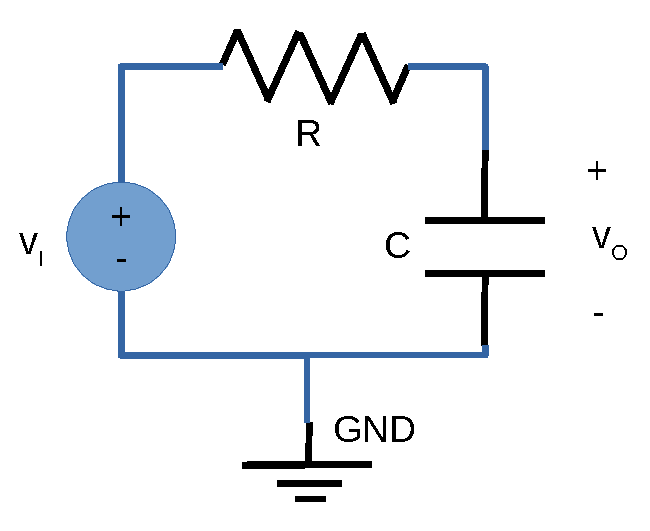
\includegraphics[width=0.6\linewidth]{rc.pdf}
  \caption{Equivalent RC circuit}
  \label{rc_fig}
\end{figure}


\subsubsection{Natural solution}

The natural solution of the capacitor behaviour is obtained by considering $v_x(t\geq0)=0$ and $v(0)=V_x$.

Is is known that:

\begin{equation}
  \begin{cases}
    KVL:\; v(t) + R_{eq} \cdot i(t) = 0 \\
    Capacitor:\; i(t) = C \cdot \frac{dv(t)}{dt}
  \end{cases}
  \label{sis}
\end{equation}

A first order linear equation arises from \ref{sis}, which can be readily solved:

\begin{equation}
  RC \cdot \frac{dv(t)}{dt} + v(t) = 0 \Rightarrow v(t) = Ae^{-\frac{t}{RC}}
\end{equation}

Applying the initial condition:

\begin{equation}
  v(0) = A = V_x
\end{equation}

The natural solution is:

\begin{equation}
  \label{nat_sol} v(t) =
  \begin{cases}
    V_x & \mbox{if } t \leq 0 \\
    V_xe^{-\frac{t}{RC}} & \mbox{if } t > 0
  \end{cases}
\end{equation}

\begin{figure}[H]
  \centering
  \includegraphics[width=0.8\linewidth]{natural.eps}
  \caption{Natural response.}
  \label{fig:nat}
\end{figure}
